\subsection{Normalized Mutual Information evolution}

	\subsubsection{NMI evolution over number of clusters for 2 zernike mode related datasets}
		\begin{figure*}[ht!]
			\centering
			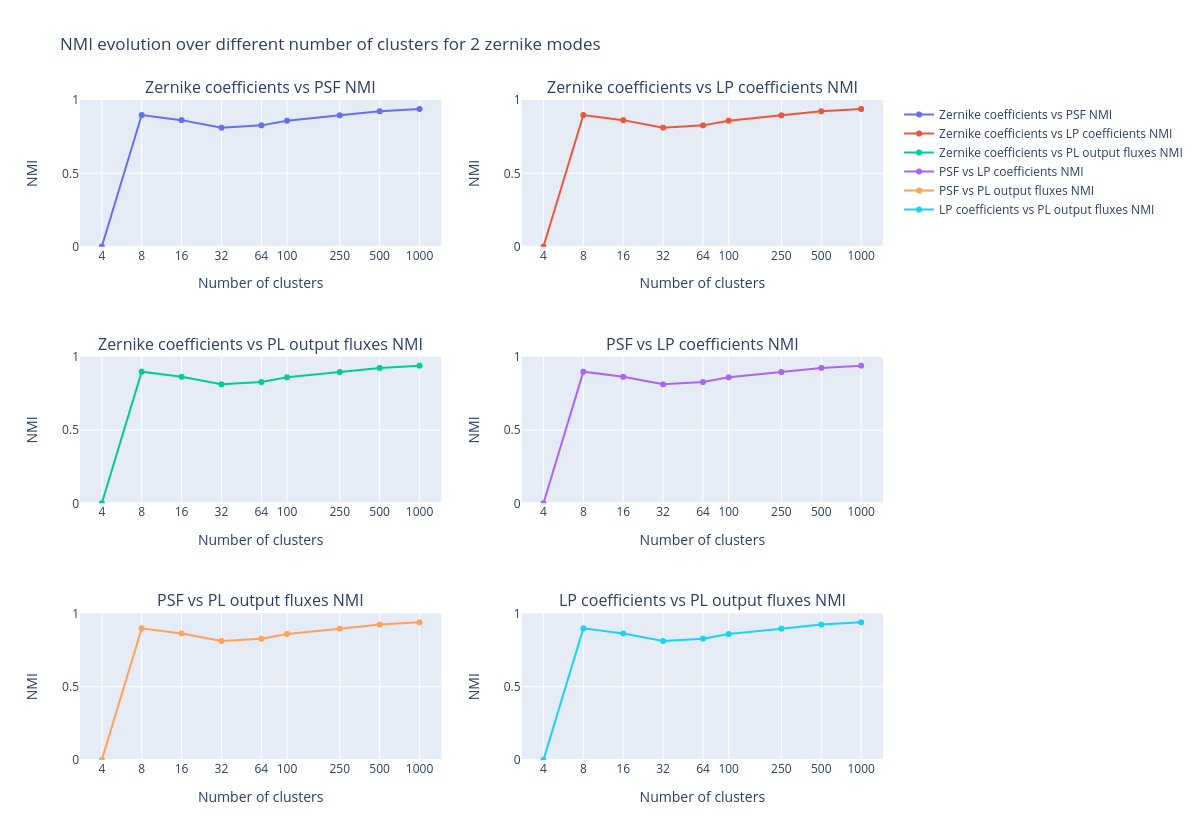
\includegraphics[width=0.9\textwidth]{nmia-nmievolutionover2.png}
		\end{figure*}
		\begin{table}[!h]
		\centering
		\begin{tabular}{|c|c|c|c|c|c|c|}
\hline
\textbf{Clusters} & \textbf{Z vs PSF} & \textbf{Z vs LP} & \textbf{Z vs PL} & \textbf{PSF vs LP} & \textbf{PSF vs PL} & \textbf{LP vs PL} \\
\hline
4   & 0.925 & 0.934 & 0.628 & 0.892 & 0.604 & 0.637 \\
8   & 0.921 & 0.910 & 0.633 & 0.892 & 0.630 & 0.649 \\
16  & 0.872 & 0.897 & 0.766 & 0.857 & 0.756 & 0.802 \\
32  & 0.793 & 0.891 & 0.770 & 0.774 & 0.759 & 0.766 \\
64  & 0.844 & 0.860 & 0.834 & 0.848 & 0.818 & 0.850 \\
100 & 0.865 & 0.875 & 0.846 & 0.863 & 0.846 & 0.861 \\
250 & 0.895 & 0.881 & 0.872 & 0.898 & 0.883 & 0.885 \\
500 & 0.919 & 0.917 & 0.905 & 0.919 & 0.908 & 0.913 \\
1000 & 0.937 & 0.943 & 0.937 & 0.933 & 0.930 & 0.942 \\
2000 & 0.959 & 0.972 & 0.965 & 0.956 & 0.952 & 0.969 \\
\hline
\end{tabular}
\caption{NMI Analysis for Different Numbers of Clusters}
\end{table}		
		\FloatBarrier
		
	\subsubsection{NMI evolution over number of clusters for 5 zernike mode related datasets}
		\begin{figure*}[ht!]
			\centering
			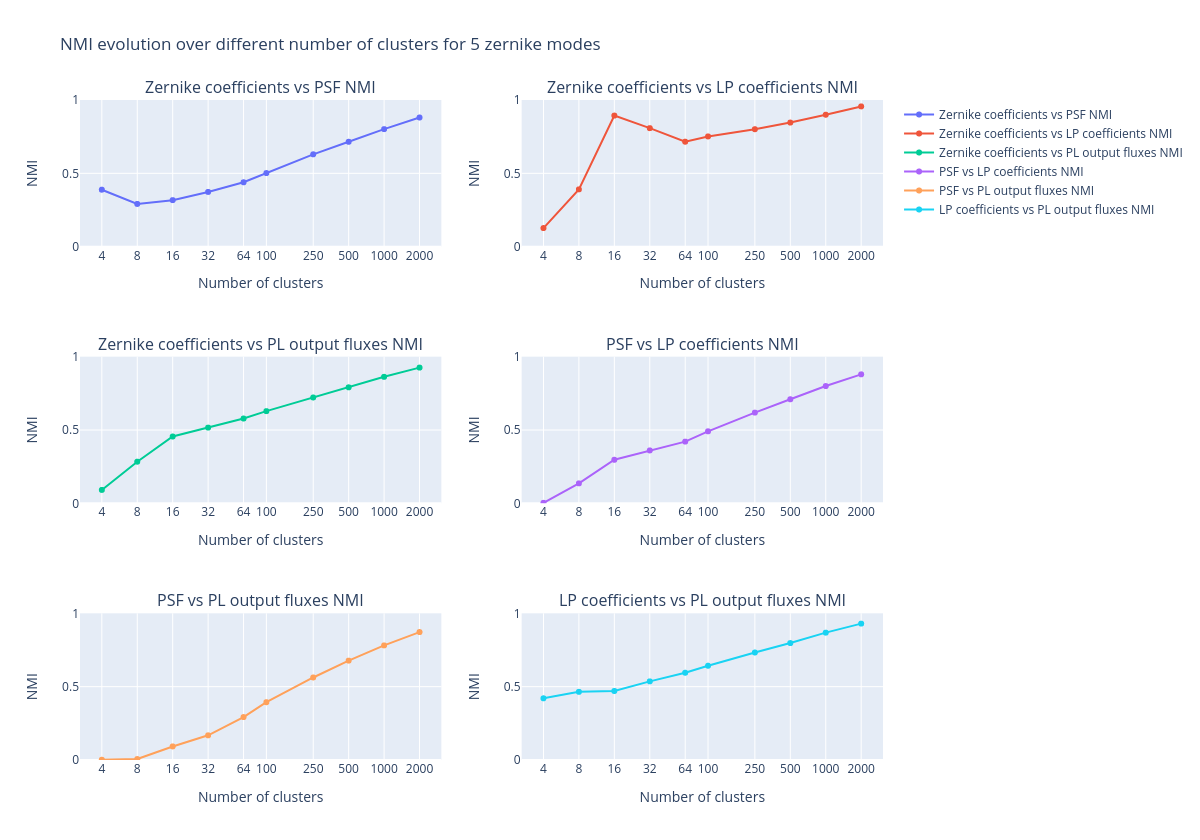
\includegraphics[width=0.9\textwidth]{nmia-nmievolutionover5.png}
		\end{figure*}
		
		\begin{table}[h!]
\centering
\begin{tabular}{|c|c|c|c|c|c|c|}
\hline
\textbf{Clusters} & \textbf{Z vs PSF} & \textbf{Z vs LP} & \textbf{Z vs PL} & \textbf{PSF vs LP} & \textbf{PSF vs PL} & \textbf{LP vs PL} \\
\hline
4  & 0.3884 & 0.1268 & 0.0914 & 0.0033 & 0.0016 & 0.4207 \\
8  & 0.2913 & 0.3905 & 0.2838 & 0.1361 & 0.0064 & 0.4649 \\
16 & 0.3172 & 0.8939 & 0.4555 & 0.2970 & 0.0925 & 0.4705 \\
32 & 0.3731 & 0.8080 & 0.5162 & 0.3606 & 0.1683 & 0.5361 \\
64 & 0.4390 & 0.7155 & 0.5783 & 0.4208 & 0.2927 & 0.5950 \\
100 & 0.5018 & 0.7515 & 0.6286 & 0.4911 & 0.3940 & 0.6427 \\
250 & 0.6296 & 0.8008 & 0.7217 & 0.6187 & 0.5626 & 0.7328 \\
500 & 0.7151 & 0.8462 & 0.7910 & 0.7095 & 0.6774 & 0.7972 \\
1000 & 0.8012 & 0.8996 & 0.8626 & 0.7995 & 0.7812 & 0.8683 \\
2000 & 0.8807 & 0.9562 & 0.9255 & 0.8795 & 0.8723 & 0.9299 \\
\hline
\end{tabular}
\caption{NMI Analysis for Different Numbers of Clusters}
\end{table}
		\FloatBarrier
		
	\subsubsection{NMI evolution over number of clusters for 9 zernike mode related datasets}
		\begin{figure*}[ht!]
			\centering
			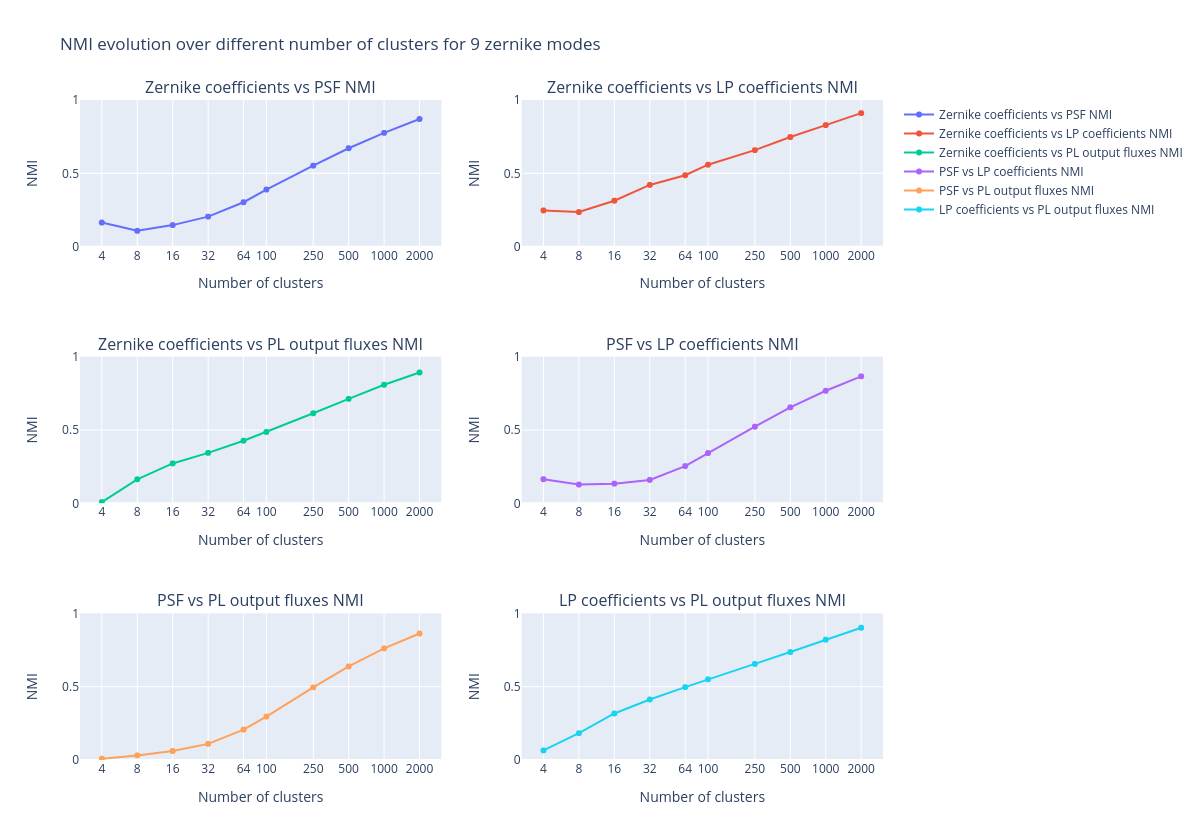
\includegraphics[width=0.9\textwidth]{nmia-nmievolutionover9.png}
		\end{figure*}

\begin{table}[h!]
\centering
\begin{tabular}{|c|c|c|c|c|c|c|}
\hline
\textbf{Clusters} & \textbf{Z vs PSF} & \textbf{Z vs LP} & \textbf{Z vs PL} & \textbf{PSF vs LP} & \textbf{PSF vs PL} & \textbf{LP vs PL} \\
\hline
4 & 0.164 & 0.247 & 0.009 & 0.165 & 0.009 & 0.065 \\
8 & 0.108 & 0.236 & 0.164 & 0.128 & 0.031 & 0.183 \\
16 & 0.147 & 0.313 & 0.272 & 0.134 & 0.061 & 0.317 \\
32 & 0.205 & 0.421 & 0.344 & 0.160 & 0.110 & 0.413 \\
64 & 0.303 & 0.487 & 0.427 & 0.254 & 0.207 & 0.497 \\
100 & 0.389 & 0.559 & 0.487 & 0.343 & 0.296 & 0.550 \\
250 & 0.552 & 0.658 & 0.614 & 0.522 & 0.495 & 0.655 \\
500 & 0.671 & 0.747 & 0.712 & 0.655 & 0.638 & 0.736 \\
1000 & 0.776 & 0.829 & 0.809 & 0.768 & 0.761 & 0.820 \\
2000 & 0.870 & 0.910 & 0.892 & 0.866 & 0.862 & 0.902 \\
\hline
\end{tabular}
\caption{NMI Analysis for Different Numbers of Clusters}
\end{table}

		\FloatBarrier
		
	\subsubsection{NMI evolution over number of clusters for 14 zernike mode related datasets}
		\begin{figure*}[ht!]
			\centering
			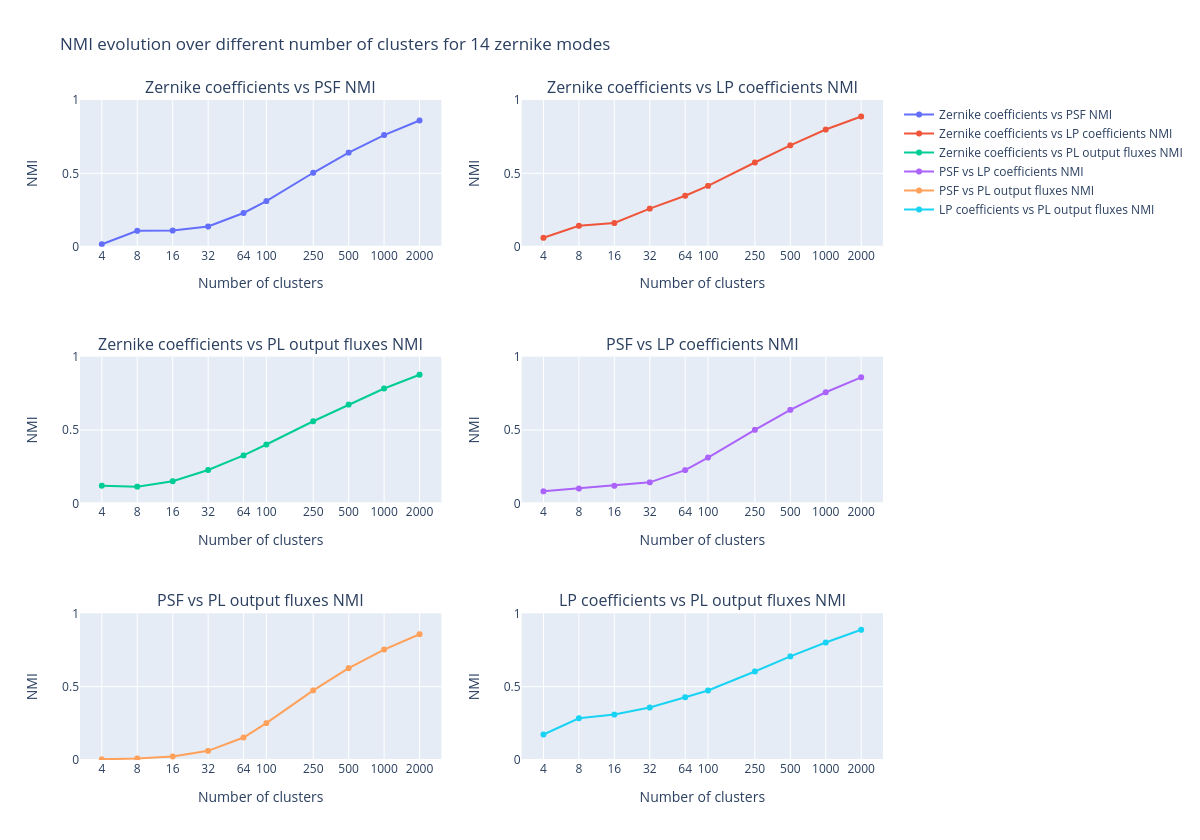
\includegraphics[width=0.9\textwidth]{nmia-nmievolutionover14.png}
		\end{figure*}
		
\begin{table}[h!]
\centering
\begin{tabular}{|c|c|c|c|c|c|c|}
\hline
\textbf{Clusters} & \textbf{Z vs PSF} & \textbf{Z vs LP} & \textbf{Z vs PL} & \textbf{PSF vs LP} & \textbf{PSF vs PL} & \textbf{LP vs PL} \\
\hline
4 & 0.017 & 0.060 & 0.120 & 0.082 & 0.004 & 0.174 \\
8 & 0.108 & 0.142 & 0.114 & 0.101 & 0.010 & 0.285 \\
16 & 0.110 & 0.161 & 0.151 & 0.120 & 0.024 & 0.310 \\
32 & 0.137 & 0.259 & 0.227 & 0.143 & 0.062 & 0.358 \\
64 & 0.230 & 0.347 & 0.327 & 0.226 & 0.153 & 0.428 \\
100 & 0.311 & 0.414 & 0.401 & 0.312 & 0.252 & 0.474 \\
250 & 0.504 & 0.574 & 0.560 & 0.501 & 0.475 & 0.604 \\
500 & 0.641 & 0.691 & 0.673 & 0.637 & 0.626 & 0.706 \\
1000 & 0.761 & 0.799 & 0.783 & 0.757 & 0.753 & 0.801 \\
2000 & 0.860 & 0.888 & 0.877 & 0.859 & 0.858 & 0.888 \\
\hline
\end{tabular}
\caption{NMI Analysis for Different Numbers of Clusters}
\end{table}
		\FloatBarrier
		
	\subsubsection{NMI evolution over number of clusters for 20 zernike mode related datasets}
		\begin{figure*}[ht!]
			\centering
			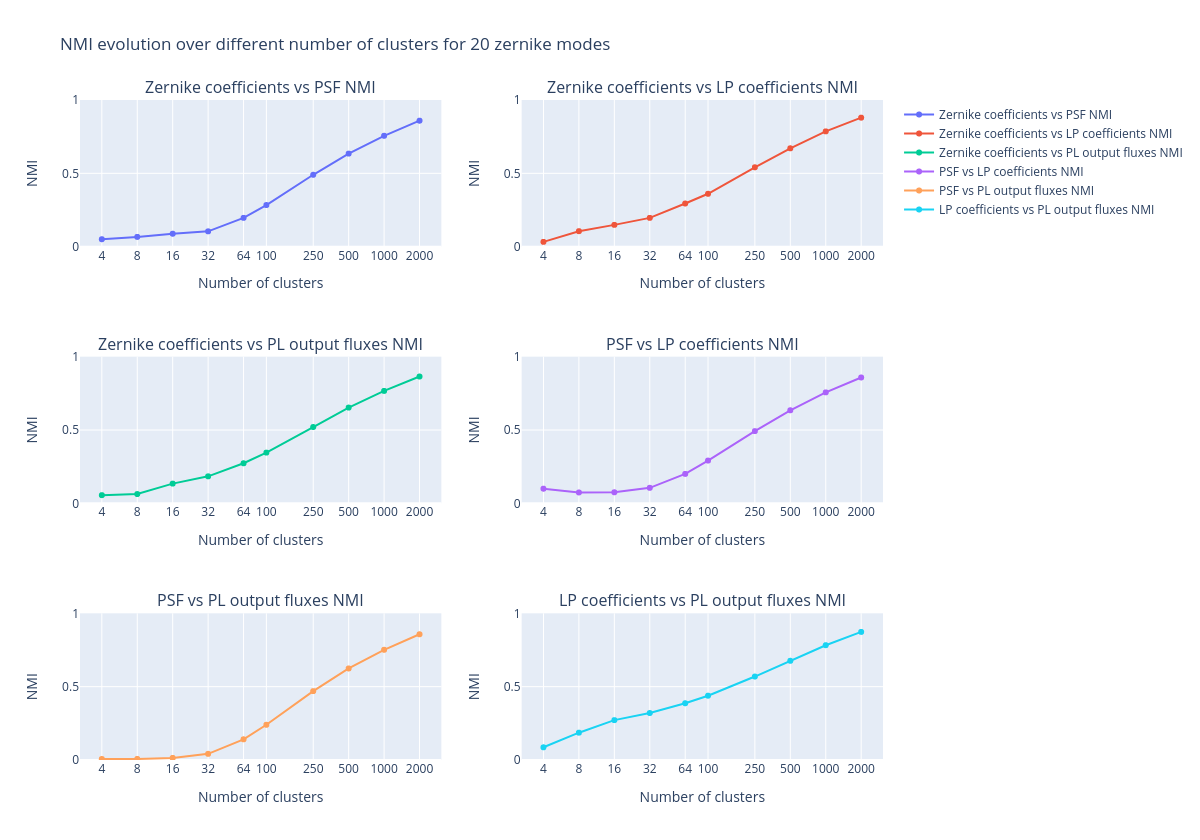
\includegraphics[width=0.9\textwidth]{nmia-nmievolutionover20.png}
		\end{figure*}
		
\begin{table}[h!]
\centering
\begin{tabular}{|c|c|c|c|c|c|c|}
\hline
\textbf{Clusters} & \textbf{Z vs PSF} & \textbf{Z vs LP} & \textbf{Z vs PL} & \textbf{PSF vs LP} & \textbf{PSF vs PL} & \textbf{LP vs PL} \\
\hline
4   & 0.051 & 0.033 & 0.056 & 0.100 & 0.007 & 0.087 \\
8   & 0.067 & 0.106 & 0.063 & 0.074 & 0.007 & 0.186 \\
16  & 0.088 & 0.149 & 0.134 & 0.075 & 0.014 & 0.272 \\
32  & 0.105 & 0.196 & 0.184 & 0.106 & 0.042 & 0.320 \\
64  & 0.196 & 0.294 & 0.273 & 0.201 & 0.141 & 0.387 \\
100 & 0.284 & 0.361 & 0.346 & 0.292 & 0.240 & 0.438 \\
250 & 0.490 & 0.541 & 0.520 & 0.492 & 0.470 & 0.569 \\
500 & 0.635 & 0.671 & 0.653 & 0.635 & 0.624 & 0.676 \\
1000 & 0.756 & 0.786 & 0.766 & 0.757 & 0.752 & 0.783 \\
2000 & 0.859 & 0.879 & 0.865 & 0.858 & 0.857 & 0.873 \\
\hline
\end{tabular}
\caption{NMI Analysis for Different Numbers of Clusters}
\end{table}
		\FloatBarrier
		
		
	\subsubsection{NMI evolution over number of clusters for 27 zernike mode related datasets}
		\begin{figure*}[ht!]
			\centering
			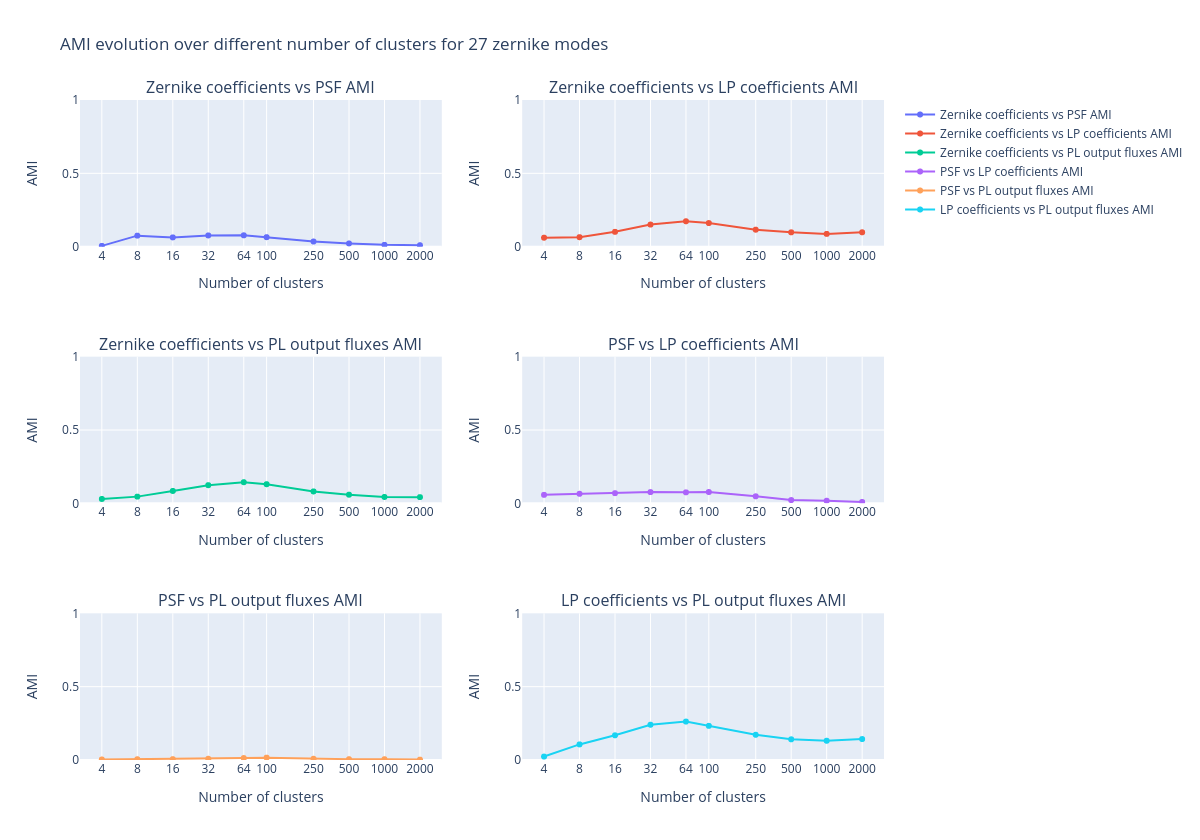
\includegraphics[width=0.9\textwidth]{nmia-nmievolutionover27.png}
		\end{figure*}
		
\begin{table}[h!]
\centering
\begin{tabular}{|c|c|c|c|c|c|c|}
\hline
\textbf{Clusters} & \textbf{Z vs PSF} & \textbf{Z vs LP} & \textbf{Z vs PL} & \textbf{PSF vs LP} & \textbf{PSF vs PL} & \textbf{LP vs PL} \\
\hline
4   & 0.006 & 0.062 & 0.030 & 0.059 & 0.004 & 0.024 \\
8   & 0.077 & 0.067 & 0.048 & 0.067 & 0.007 & 0.108 \\
16  & 0.071 & 0.108 & 0.092 & 0.077 & 0.014 & 0.175 \\
32  & 0.104 & 0.175 & 0.149 & 0.104 & 0.037 & 0.263 \\
64  & 0.180 & 0.265 & 0.239 & 0.177 & 0.123 & 0.344 \\
100 & 0.264 & 0.341 & 0.317 & 0.274 & 0.226 & 0.397 \\
250 & 0.477 & 0.522 & 0.503 & 0.485 & 0.463 & 0.552 \\
500 & 0.626 & 0.656 & 0.640 & 0.627 & 0.620 & 0.672 \\
1000 & 0.750 & 0.767 & 0.755 & 0.752 & 0.749 & 0.778 \\
2000 & 0.855 & 0.865 & 0.857 & 0.856 & 0.855 & 0.872 \\
\hline
\end{tabular}
\caption{NMI Analysis for Different Numbers of Clusters}
\end{table}
		\FloatBarrier
		
	
	\subsubsection{NMI evolution over number of clusters for 35 zernike mode related datasets}
		\begin{figure*}[ht!]
			\centering
			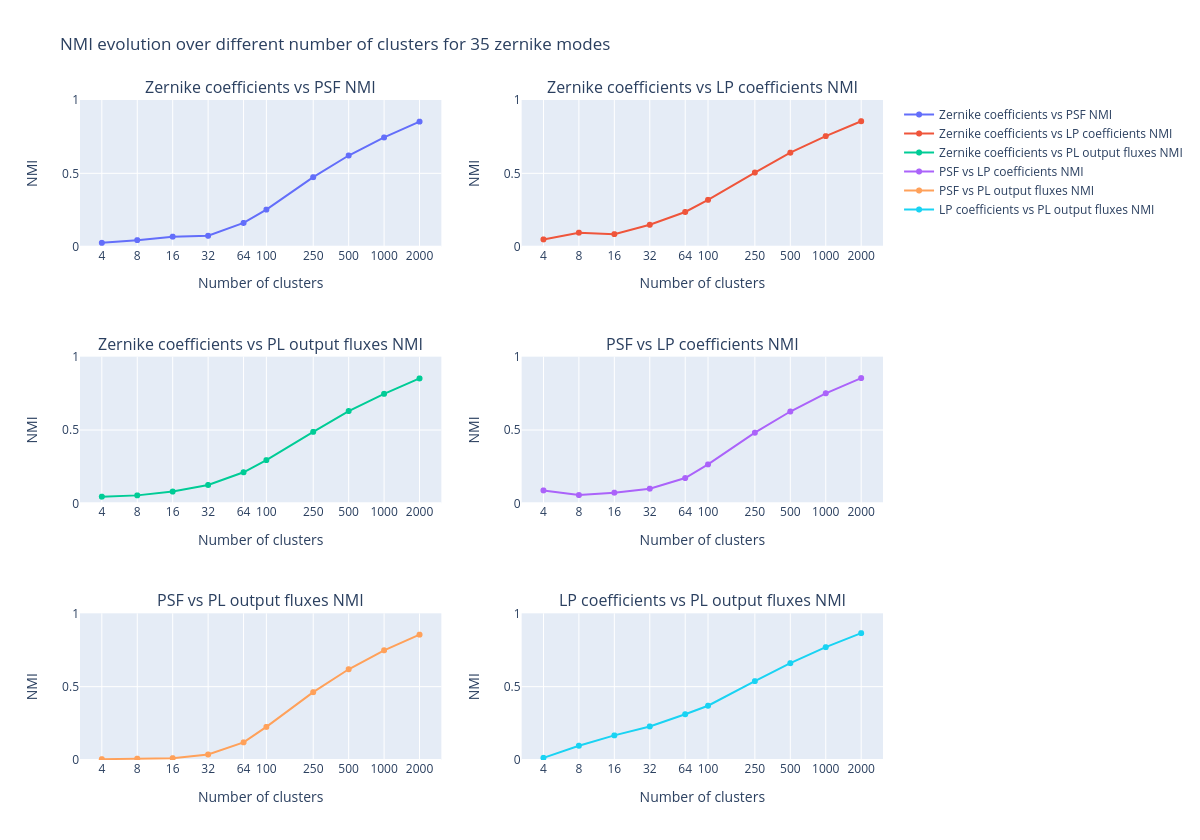
\includegraphics[width=0.9\textwidth]{nmia-nmievolutionover35.png}
		\end{figure*}
		
\begin{table}[h!]
\centering
\begin{tabular}{|c|c|c|c|c|c|c|}
\hline
\textbf{Clusters} & \textbf{Z vs PSF} & \textbf{Z vs LP} & \textbf{Z vs PL} & \textbf{PSF vs LP} & \textbf{PSF vs PL} & \textbf{LP vs PL} \\
\hline
4   & 0.026 & 0.049 & 0.046 & 0.088 & 0.006 & 0.015 \\
8   & 0.045 & 0.095 & 0.054 & 0.056 & 0.009 & 0.097 \\
16  & 0.068 & 0.085 & 0.080 & 0.073 & 0.013 & 0.168 \\
32  & 0.074 & 0.149 & 0.125 & 0.100 & 0.037 & 0.229 \\
64  & 0.162 & 0.236 & 0.212 & 0.172 & 0.120 & 0.312 \\
100 & 0.253 & 0.319 & 0.295 & 0.265 & 0.226 & 0.370 \\
250 & 0.474 & 0.506 & 0.487 & 0.482 & 0.462 & 0.538 \\
500 & 0.622 & 0.641 & 0.629 & 0.626 & 0.619 & 0.660 \\
1000 & 0.745 & 0.754 & 0.747 & 0.750 & 0.748 & 0.769 \\
2000 & 0.853 & 0.855 & 0.852 & 0.854 & 0.855 & 0.865 \\
\hline
\end{tabular}
\caption{NMI Analysis for Different Numbers of Clusters}
\end{table}
		\FloatBarrier
		
		
	\subsubsection{NMI evolution over number of clusters for 44 zernike mode related datasets}
		\begin{figure*}[ht!]
			\centering
			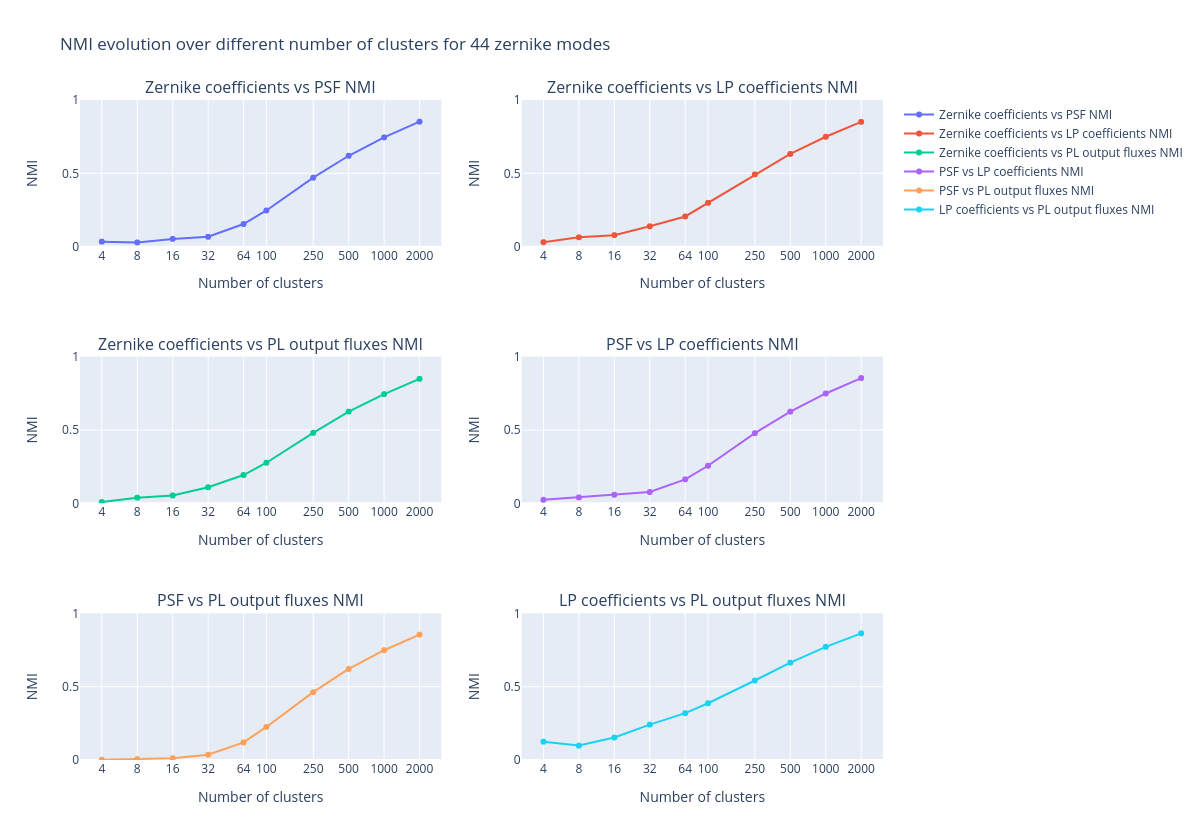
\includegraphics[width=0.9\textwidth]{nmia-nmievolutionover44.png}
		\end{figure*}
		
\begin{table}[h!]
\centering
\begin{tabular}{|c|c|c|c|c|c|c|}
\hline
\textbf{Clusters} & \textbf{Z vs PSF} & \textbf{Z vs LP} & \textbf{Z vs PL} & \textbf{PSF vs LP} & \textbf{PSF vs PL} & \textbf{LP vs PL} \\
\hline
4   & 0.034 & 0.031 & 0.009 & 0.024 & 0.002 & 0.125 \\
8   & 0.029 & 0.064 & 0.039 & 0.040 & 0.006 & 0.098 \\
16  & 0.053 & 0.079 & 0.054 & 0.058 & 0.012 & 0.153 \\
32  & 0.067 & 0.139 & 0.110 & 0.077 & 0.036 & 0.241 \\
64  & 0.155 & 0.206 & 0.193 & 0.164 & 0.120 & 0.320 \\
100 & 0.247 & 0.299 & 0.277 & 0.256 & 0.225 & 0.387 \\
250 & 0.470 & 0.493 & 0.481 & 0.478 & 0.463 & 0.542 \\
500 & 0.620 & 0.632 & 0.625 & 0.625 & 0.621 & 0.664 \\
1000 & 0.745 & 0.749 & 0.745 & 0.749 & 0.749 & 0.772 \\
2000 & 0.852 & 0.851 & 0.849 & 0.854 & 0.855 & 0.864 \\
\hline
\end{tabular}
\caption{NMI Analysis for Different Numbers of Clusters}
\end{table}
		\FloatBarrier
		
		
	\subsubsection{NMI evolution over number of zernike modes}
	
	\begin{figure*}[ht!]
			\centering
			\subfloat[NMI evolution over number of clusters for Zernike coefficients vs PSF]{%
				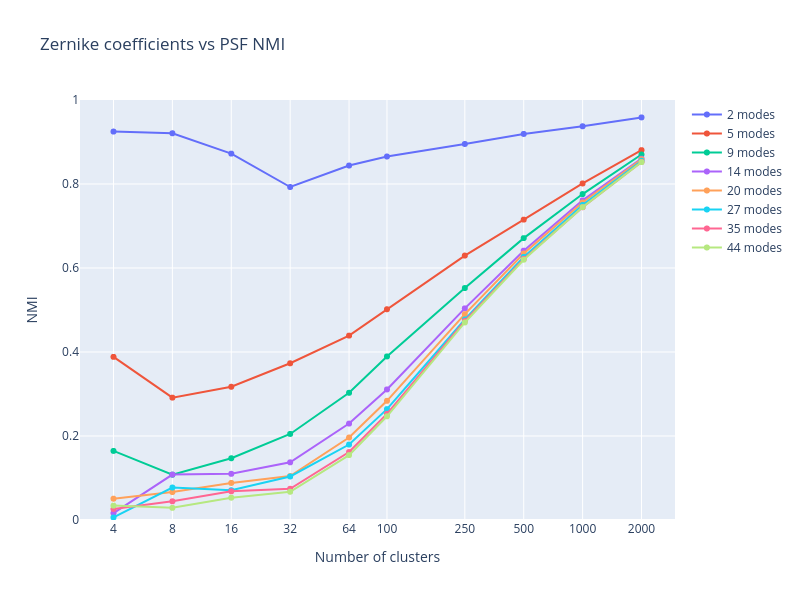
\includegraphics[width=0.45\textwidth]{nmia-zernikecoefficientsvspsfnmi.png}}
			\hspace{\fill}
			\subfloat[NMI evolution over number of clusters for Zernike coefficients vs LP coefficients]{%
				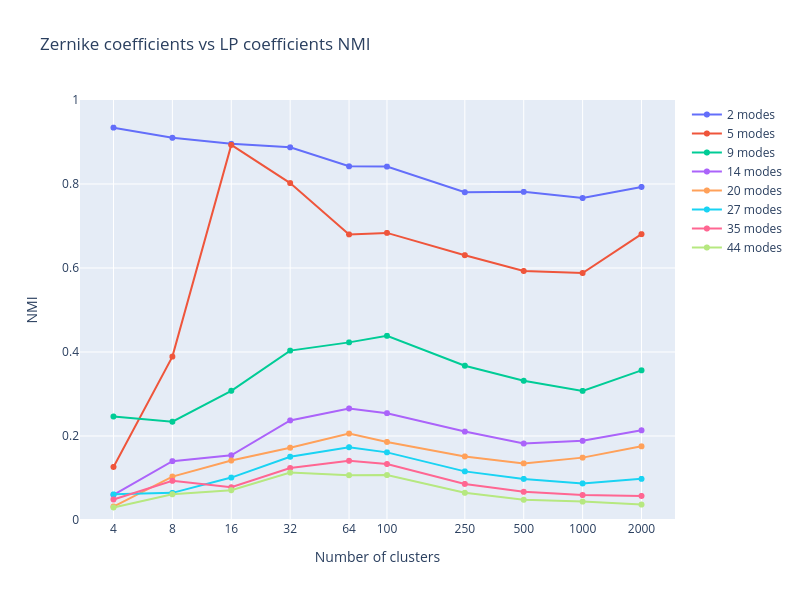
\includegraphics[width=0.45\textwidth]{nmia-zernikecoefficientsvslpcoefficientsnmi.png}}
			\\
			\subfloat[NMI evolution over number of clusters for Zernike coefficients vs PL output fluxes]{%
				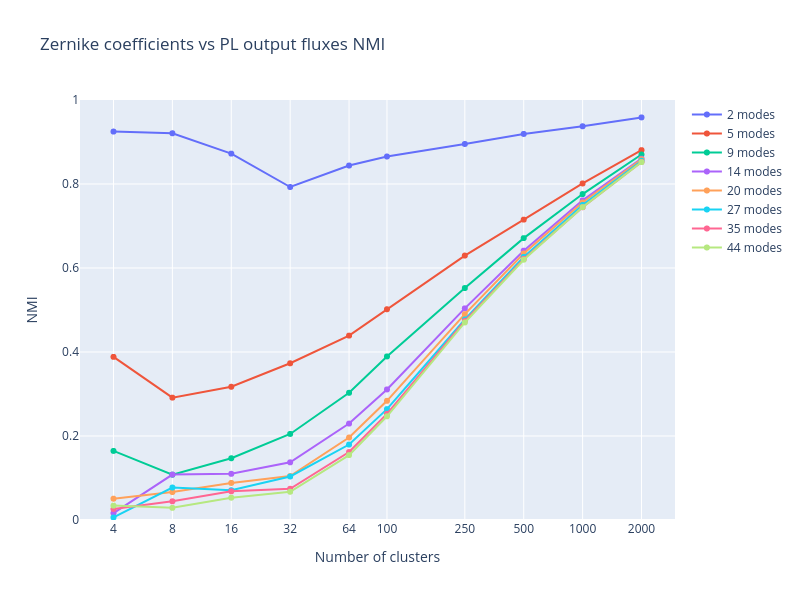
\includegraphics[width=0.45\textwidth]{nmia-zernikecoefficientsvsploutputfluxesnmi.png}}
			\hspace{\fill}
			\subfloat[NMI evolution over number of clusters for PSF vs LP coefficients]{%
				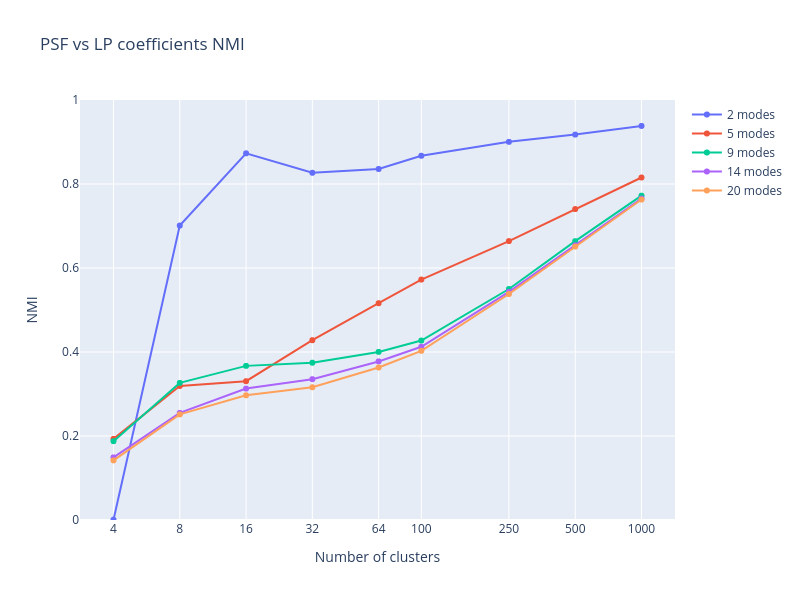
\includegraphics[width=0.45\textwidth]{nmia-psfvslpcoefficientsnmi.png}}
			\\
			\subfloat[NMI evolution over number of clusters for PSF vs PL output fluxes]{%
				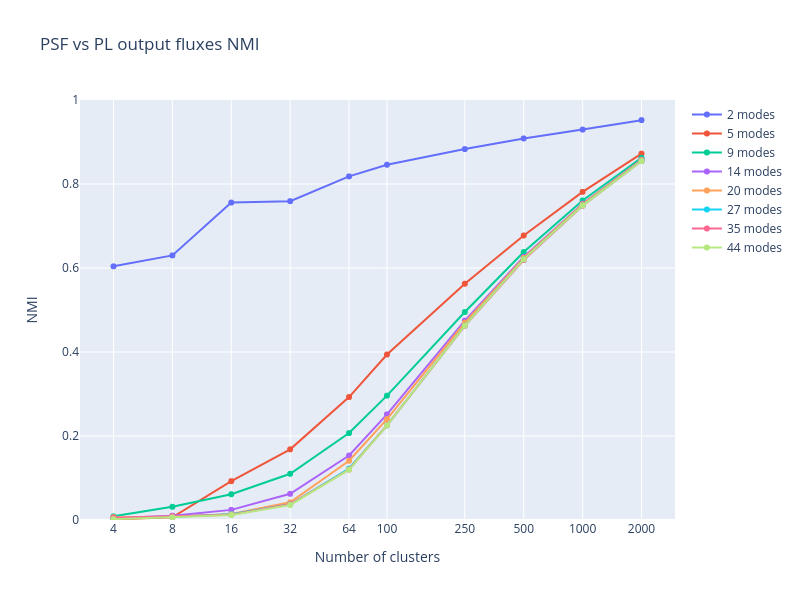
\includegraphics[width=0.45\textwidth]{nmia-psfvsploutputfluxesnmi.png}}
			\hspace{\fill}
			\subfloat[NMI evolution over number of clusters for LP coefficients vs PL output fluxes]{%
				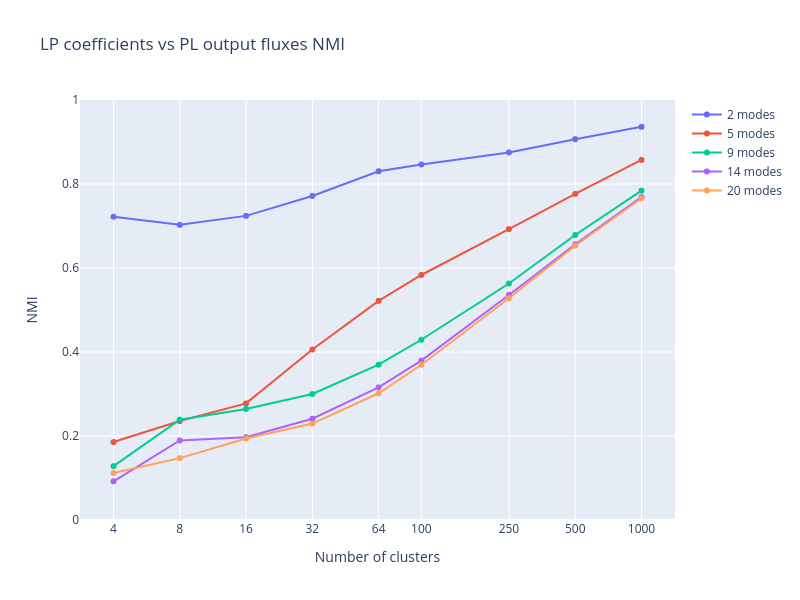
\includegraphics[width=0.45\textwidth]{nmia-lpcoefficientsvsploutputfluxesnmi.png}}
		\end{figure*}
		

		\FloatBarrier